\documentclass[titlepage,a4paper]{article}

\usepackage{a4wide}
\usepackage[colorlinks=true,linkcolor=black,urlcolor=blue,bookmarksopen=true]{hyperref}
\usepackage{bookmark}
\usepackage{fancyhdr}
\usepackage[spanish]{babel}
\usepackage[utf8]{inputenc}
\usepackage[T1]{fontenc}
\usepackage{graphicx}
\usepackage{float}

\pagestyle{fancy}
\fancyhf{}
\fancyhead[L]{TP2 - AlgoCraft}
\fancyhead[R]{Algoritmos y Programación III - FIUBA}
\renewcommand{\headrulewidth}{0.4pt}
\fancyfoot[C]{\thepage}
\renewcommand{\footrulewidth}{0.4pt}

\begin{document}
\begin{titlepage}
	\hfill
\includegraphics[width=6cm]{logofiuba.jpg}
    \centering
    \vfill
    \Huge \textbf{Trabajo Práctico 2 — AlgoCraft}
    \vskip2cm
    \Large [7507/9502] Algoritmos y Programación III\\
    Curso 1 \\
    Primer cuatrimestre de 2019 
    \vfill
   \begin{tabular}{ |l|l|l| }
		\hline
		\multicolumn{3} { |c| } {\textbf{Integrantes del grupo}} \\ \hline
		 DAVEREDE Agustín & 98540 & agusdavi64@gmail.com\\ \hline
	 	HUENUL Matías & 102135 & matias.huenul.07@gmail.com\\ \hline
		HUZAN Hugo & 67910 & hhuzan@gmail.com\\ \hline
		LAMPROPULOS Santiago & 101862 & santiagolampropulos@gmail.com\\ \hline
\end{tabular}
    \vfill
    \vfill
\end{titlepage}

\tableofcontents
\newpage

\section{Introducción}\label{sec:intro}
El objetivo del presente trabajo práctico fue crear una aplicación basada en el videojuego \emph{Minecraft}, que permitiera al jugador explorar un mapa bidimensional, recolectar materiales y fabricar herramientas. La aplicación fue desarrollada en lenguaje \emph{Java}, utilizando \emph{JavaFX},  siguiendo el paradigma orientado a objetos. El diseño de la misma se basa en el patrón MVC (\emph{modelo vista controlador}). En el presente informe, que pretende servir como documentación, se exponen los conceptos teóricos utilizados y se detallan los puntos principales de la implementación.


\section{Supuestos}\label{sec:supuestos}
Debido a detalles no especificados en la consigna del trabajo práctico, se ha decidido adoptar los siguientes supuestos.
\begin{itemize}
\item La cantidad de materiales posibles a recolectar es limitada debido a que el mapa consiste de una única pantalla. Debido a esto, se decidió no poner límites a la capacidad de los inventarios del jugador.
\item En caso de que el jugador se quede sin herramientas, perderá el juego.
\end{itemize}


\section{Modelo de dominio}\label{sec:modelo}
Las principales clases del modelo son las siguientes.
\begin{description}
\item[MineCraft] Es la clase que se ocupa del armado del mapa, creación del jugador y materiales, y de actualizar el estado del juego.
\item[Jugador] Modela al jugador de la partida, que puede moverse en el mapa del juego. Posee un inventario de herramientas y materiales. Puede recolectar materiales y luego usarlos para fabricar herramientas.
\item[Mapa] Modela al mundo en el cual el jugador puede moverse. El mapa es un conjunto de celdas, las cuales pueden estar vacías o ocupadas, ya sea por el jugador o por distintos materiales.
\item[Herramienta] Es una clase abstracta que modela una herramienta genérica. Posee una durabilidad y una fuerza determinadas por el tipo específico de herramienta. Puede ser usada en materiales, reduciendo la durabilidad de éstos y también la propia.
\item[Material] Es una clase abstracta que modela un material. Posee una durabilidad, que puede ser desgastada por una herramienta. Se encuentran distribuidas en el mapa del juego y al reducirse por completo su durabilidad puede ser obtenida por el jugador.
\item[FabricadorHerramientas] Modela al mecanismo por el cual el jugador puede fabricar herramientas a partir de materiales recolectados. Posee patrones de construcción que se utilizan para crear distintos tipos de herramientas.
\item[InventarioMateriales] Modela un inventario que almacena materiales, organizándolos según el tipo.
\item[InventarioHerramientas] Modela un inventario que almacena herramientas. Se inicializa con una herramienta por defecto.
\end{description}

\section{Diagramas de clase}\label{sec:diagramasdeclase}
A continuación se encuentran los diagramas que muestran las clases implementadas y cómo se relacionan entre sí.

\begin{figure}[H]
\centering
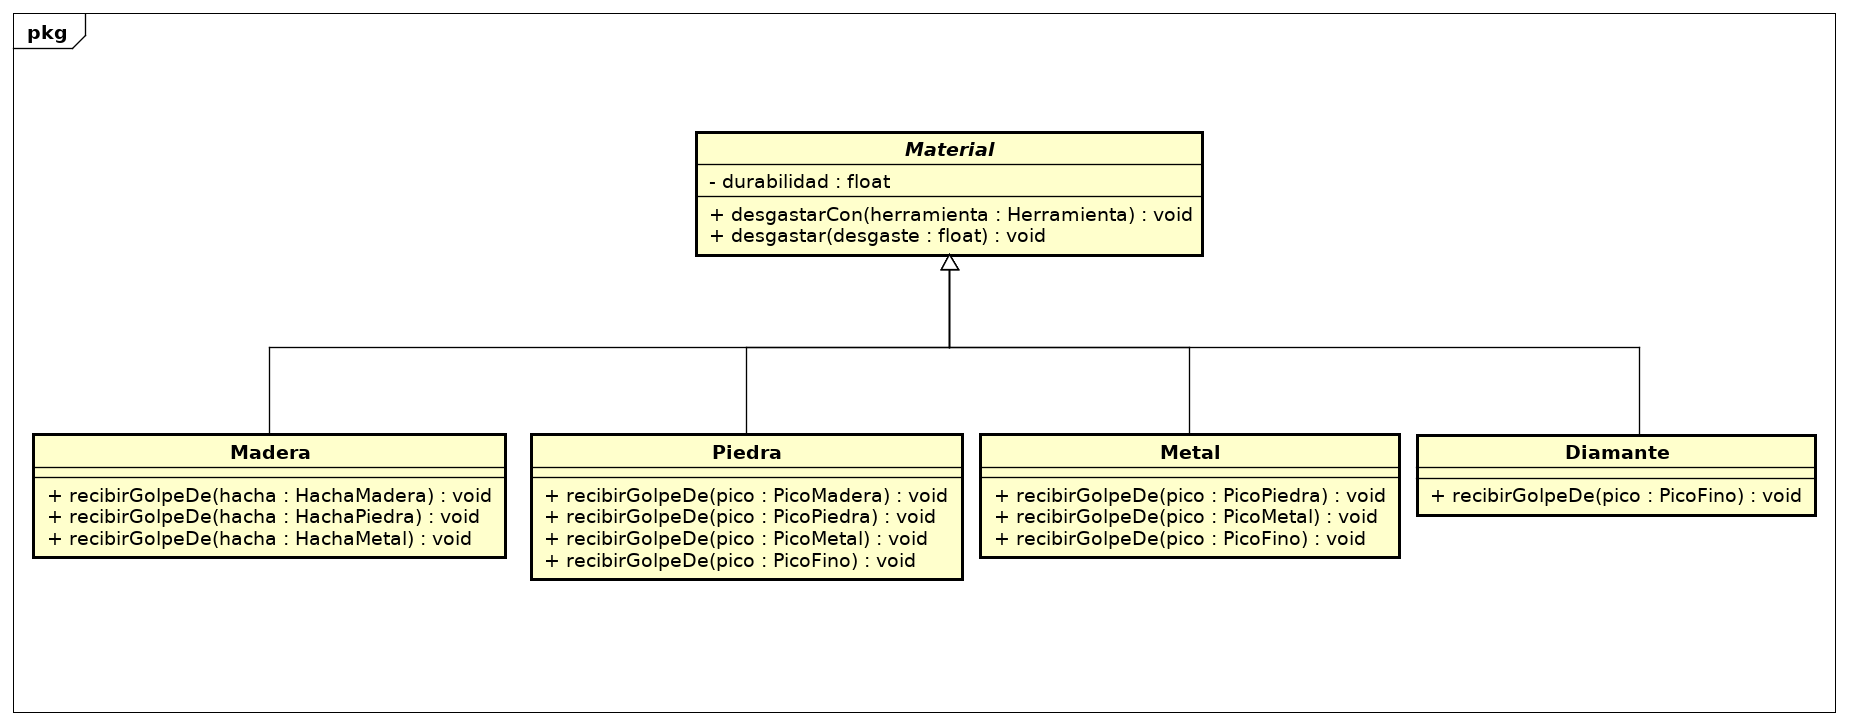
\includegraphics[width=\textwidth]{Diagramas/Materiales.png}
\caption{\label{fig:material}Diagrama de clases de Material.}
\end{figure}

\begin{figure}[H]
\centering
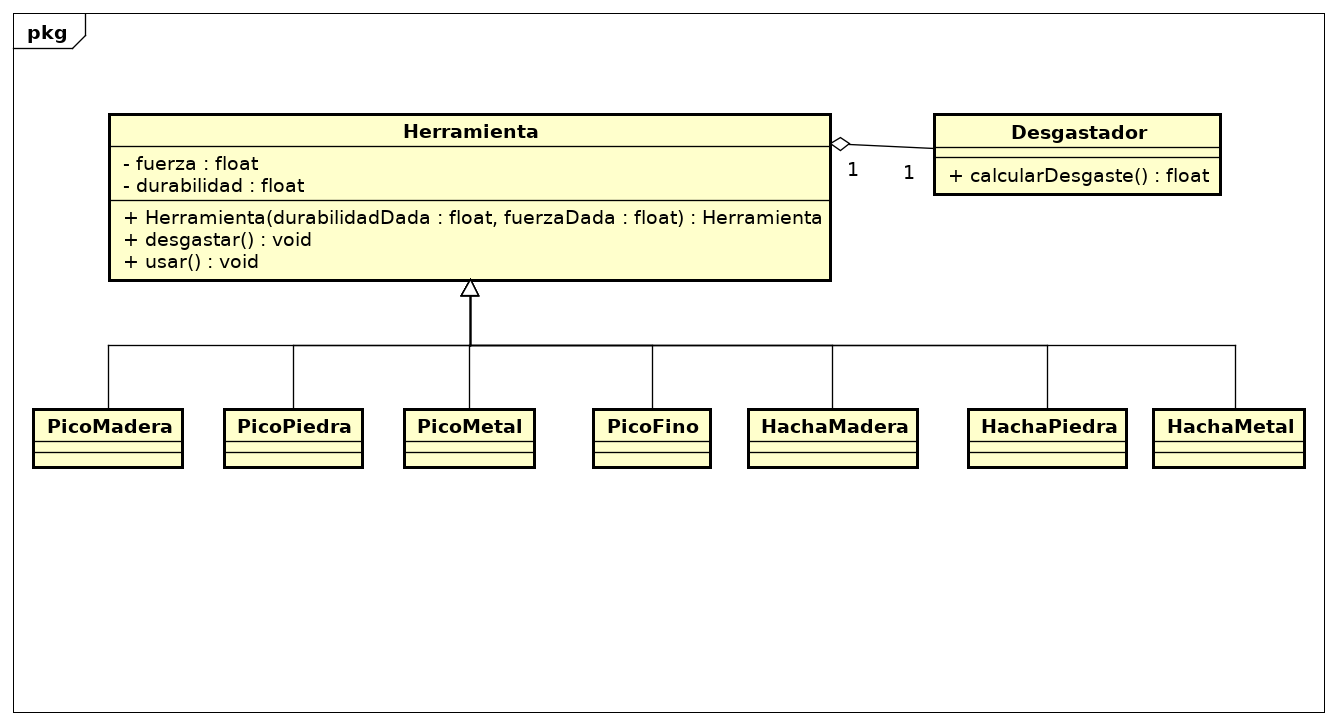
\includegraphics[width=\textwidth]{Diagramas/Herramienta.png}
\caption{\label{fig:herramienta}Diagrama de clases de Herramienta.}
\end{figure}

\begin{figure}[H]
\centering
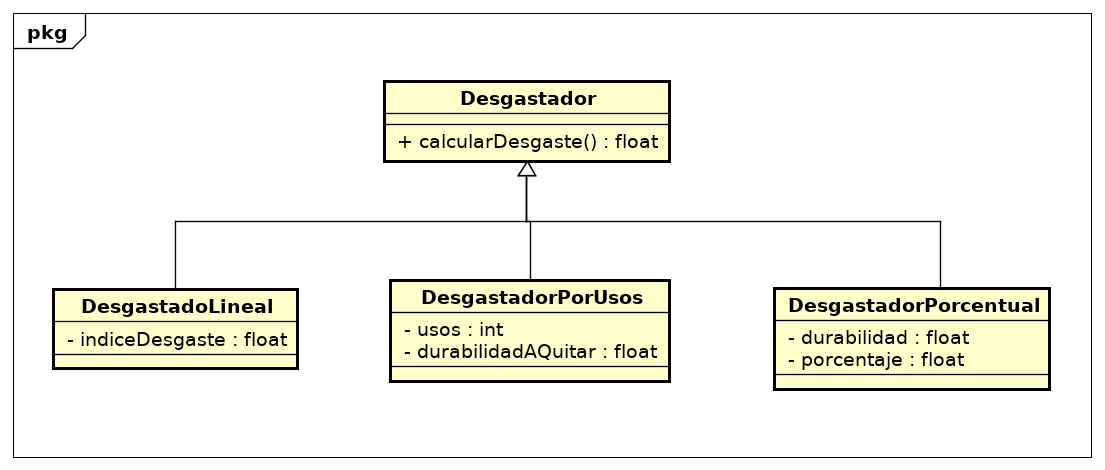
\includegraphics[width=\textwidth]{Diagramas/Desgastador.png}
\caption{\label{fig:desgastador}Diagrama de clases de Desgastador.}
\end{figure}

\begin{figure}[H]
\centering
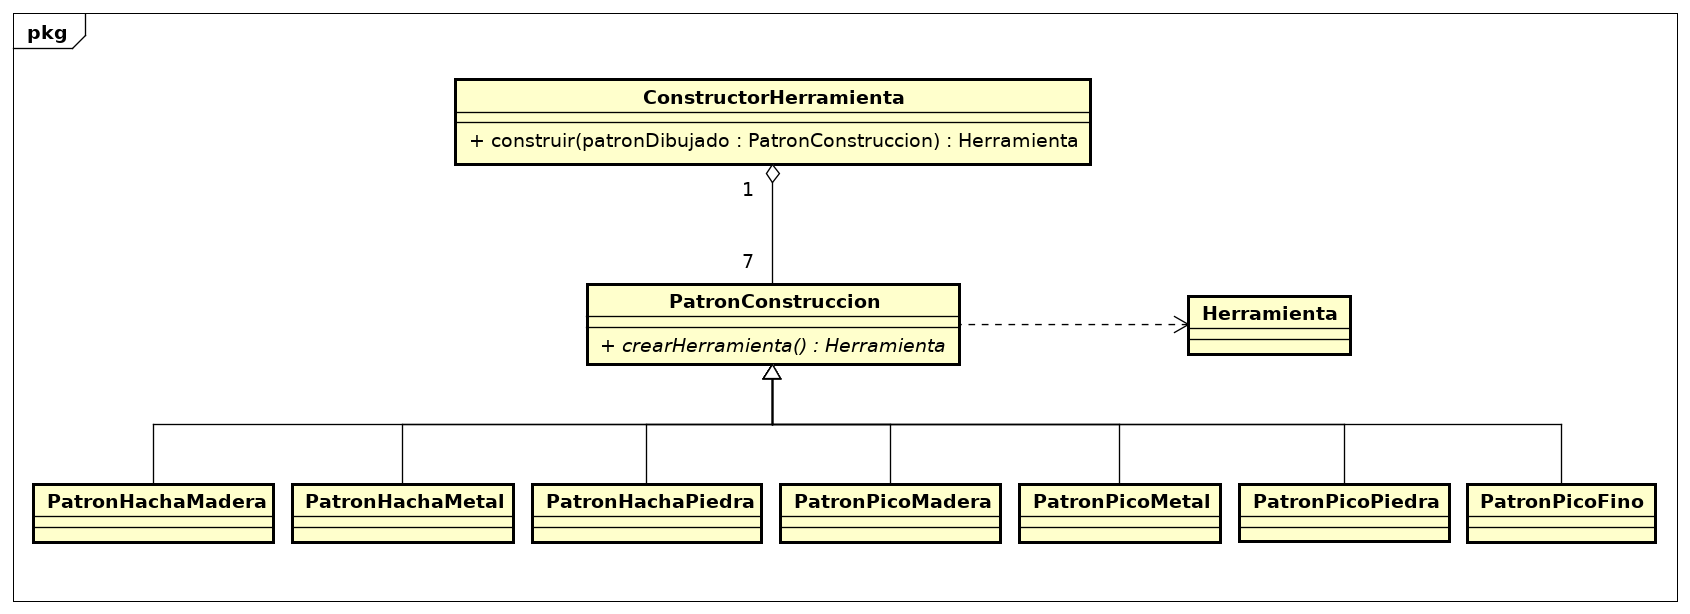
\includegraphics[width=\textwidth]{Diagramas/ConstructorHerramienta.png}
\caption{\label{fig:constructor}Diagrama de clases de ConstructorHerramienta.}
\end{figure}

\begin{figure}[H]
\centering
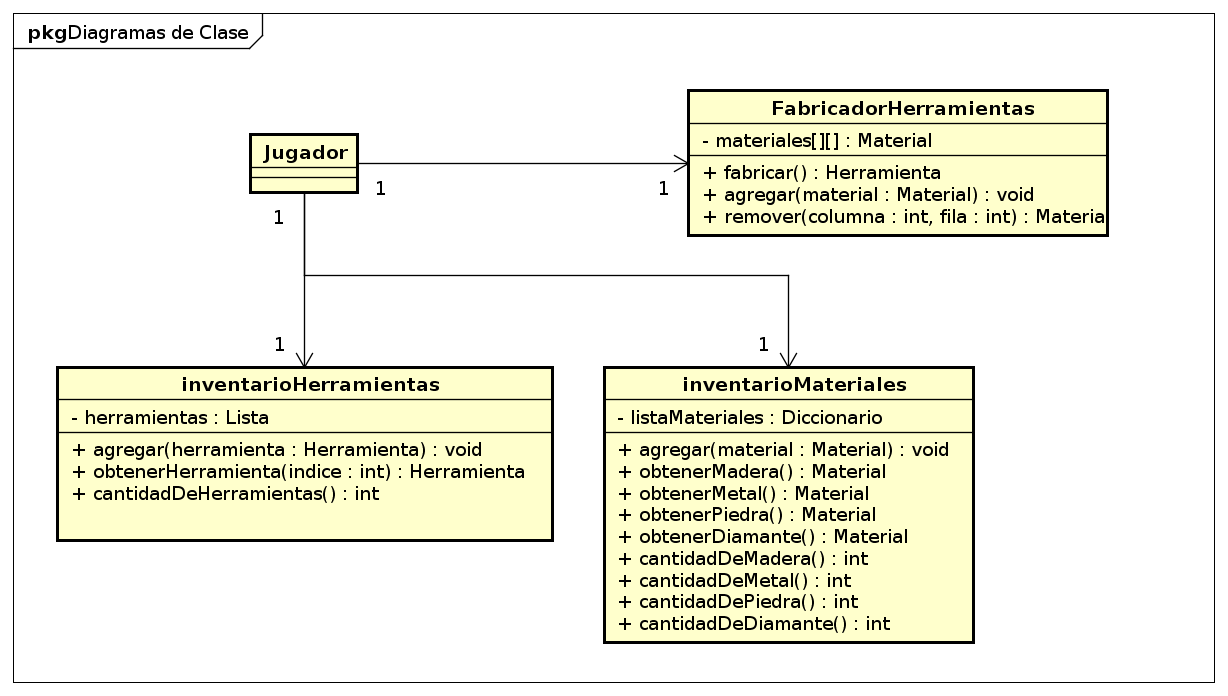
\includegraphics[width=\textwidth]{Diagramas/Personaje.png}
\caption{\label{fig:jugador}Diagrama de clases de Jugador.}
\end{figure}

\begin{figure}[H]
\centering
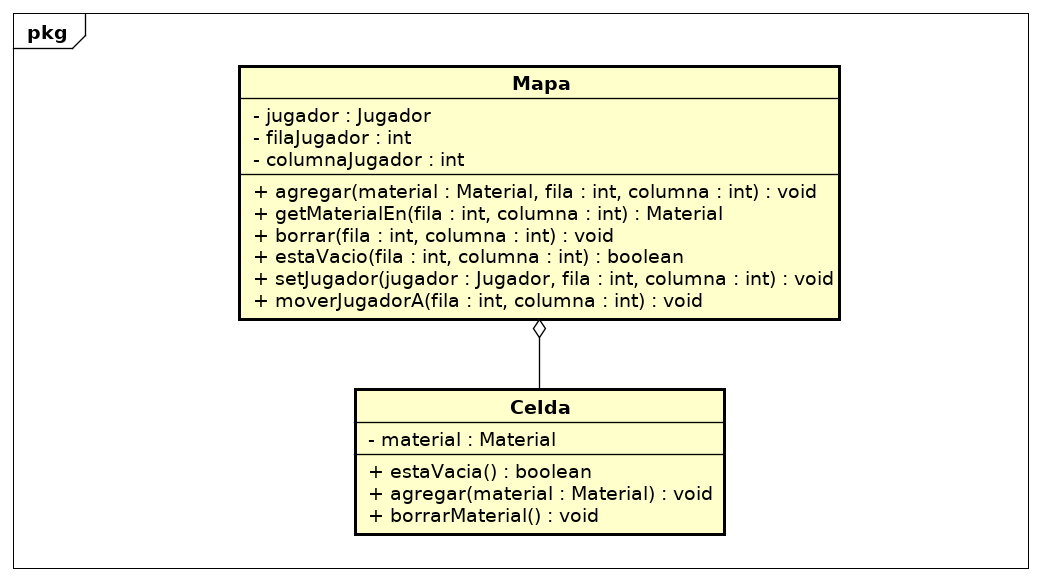
\includegraphics[width=\textwidth]{Diagramas/Mapa.png}
\caption{\label{fig:mapa}Diagrama de clases de Mapa.}
\end{figure}

\section{Detalles de implementación}\label{sec:implementacion}
En esta sección se detallarán puntos importantes de la implementación, comentando cuestiones que surgieron en el desarrollo del programa y como fueron solucionadas.
\subsection{Interacción jugador-material}
	Uno de los primeros problemas que surgieron al encarar este trabajo práctico fue definir cómo lograr que cada material pueda ser desgastado sólo por los correspondientes tipos de herramientas. Una opción era que cada material pregunte primero que clase de herramienta lo está golpeando y en base a eso decidir si se desgasta o no. Sin embargo, esta solución suponía utilizar muchos \emph{if} y además no resultaba muy apropiada en el paradigma de objetos. Entonces, se decidió utilizar la técnica de \emph{double dispatch}. De esta forma, cada material posee un método por defecto para recibir un golpe de una herramienta genérica que no modifica su durabilidad y luego se redefine este método con cada tipo de herramienta que sí puede dañar al material.
\subsection{Inventarios}
	Los inventarios de materiales y herramientas tienen comportamiento distinto.\\Por un lado, se tiene el \textbf{inventario de materiales}: al jugador no le interesa qué material en particular está eligiendo, si no sólo su tipo (todos los materiales de un mismo tipo son equivalentes), y ya que el número de materiales recolectados puede ser en principio muy grande como para disponerlos en una lista, se decidió implementarlo como un diccionario donde las claves son el tipo y los valores, \emph{ArrayLists} con las unidades de materiales. De esta forma, lo que se ve en pantalla es un casillero por tipo de material con la cantidad recolectada de cada tipo.\\
Por otro lado, el \textbf{inventario de herramientas}: cada herramienta es única en cuanto a su estado en un determinado momento (todas pueden tener distintas durabilidades) y debido a que el jugador debe ser capaz de elegir exactamente qué herramienta desea utilizar, se decidió implementarlo como un \emph{ArrayList} de herramientas. También justifica esta elección el hecho de que el inventario de herramientas tiene una capacidad menor y pre-fijada, por lo cual tiene sentido poder mostrar todas las herramientas disponibles en pantalla.
\subsection{Fabricación de herramientas}
	En el caso de la fabricación de herramientas, el jugador debe poder crearlas sólo si se agregan los materiales en un patrón específico. Para esto, se creó una clase \emph{FabricadorHerramientas} que contiene distintos patrones pre-establecidos, de clase \emph{PatronConstruccion}: cada clase derivada de esta última posee un método \emph{fabricar()} que devuelve una instancia del tipo de herramienta correspondiente. Así, cuando se ingresa un patrón, el fabricador puede compararlo con los patrones existentes y en caso de coincidir con alguno de ellos, ejecuta su método.

\section{Excepciones}\label{sec:excepciones}
\begin{description}
	\item[NoHayMaterialException] Se lanza cuando se intenta quitar un tipo de material del inventario del que no quedan unidades.
	\item[EspacioOcupadoException] Se lanza cuando se intenta agregar un material en un espacio ocupado en el fabricador de herramientas.
	\item[FabricacionNoValidaException] Se lanza cuando se intenta construir una herramienta con un patrón no existente.
	\item[GameOverException] Se lanza cuando el jugador pierde la partida por quedarse sin herramientas.
\end{description}

\section{Diagramas de secuencia}\label{sec:diagramasdesecuencia}
A continuación se presentan diagramas de algunas secuencias importantes del juego.

\begin{figure}[H]
\centering
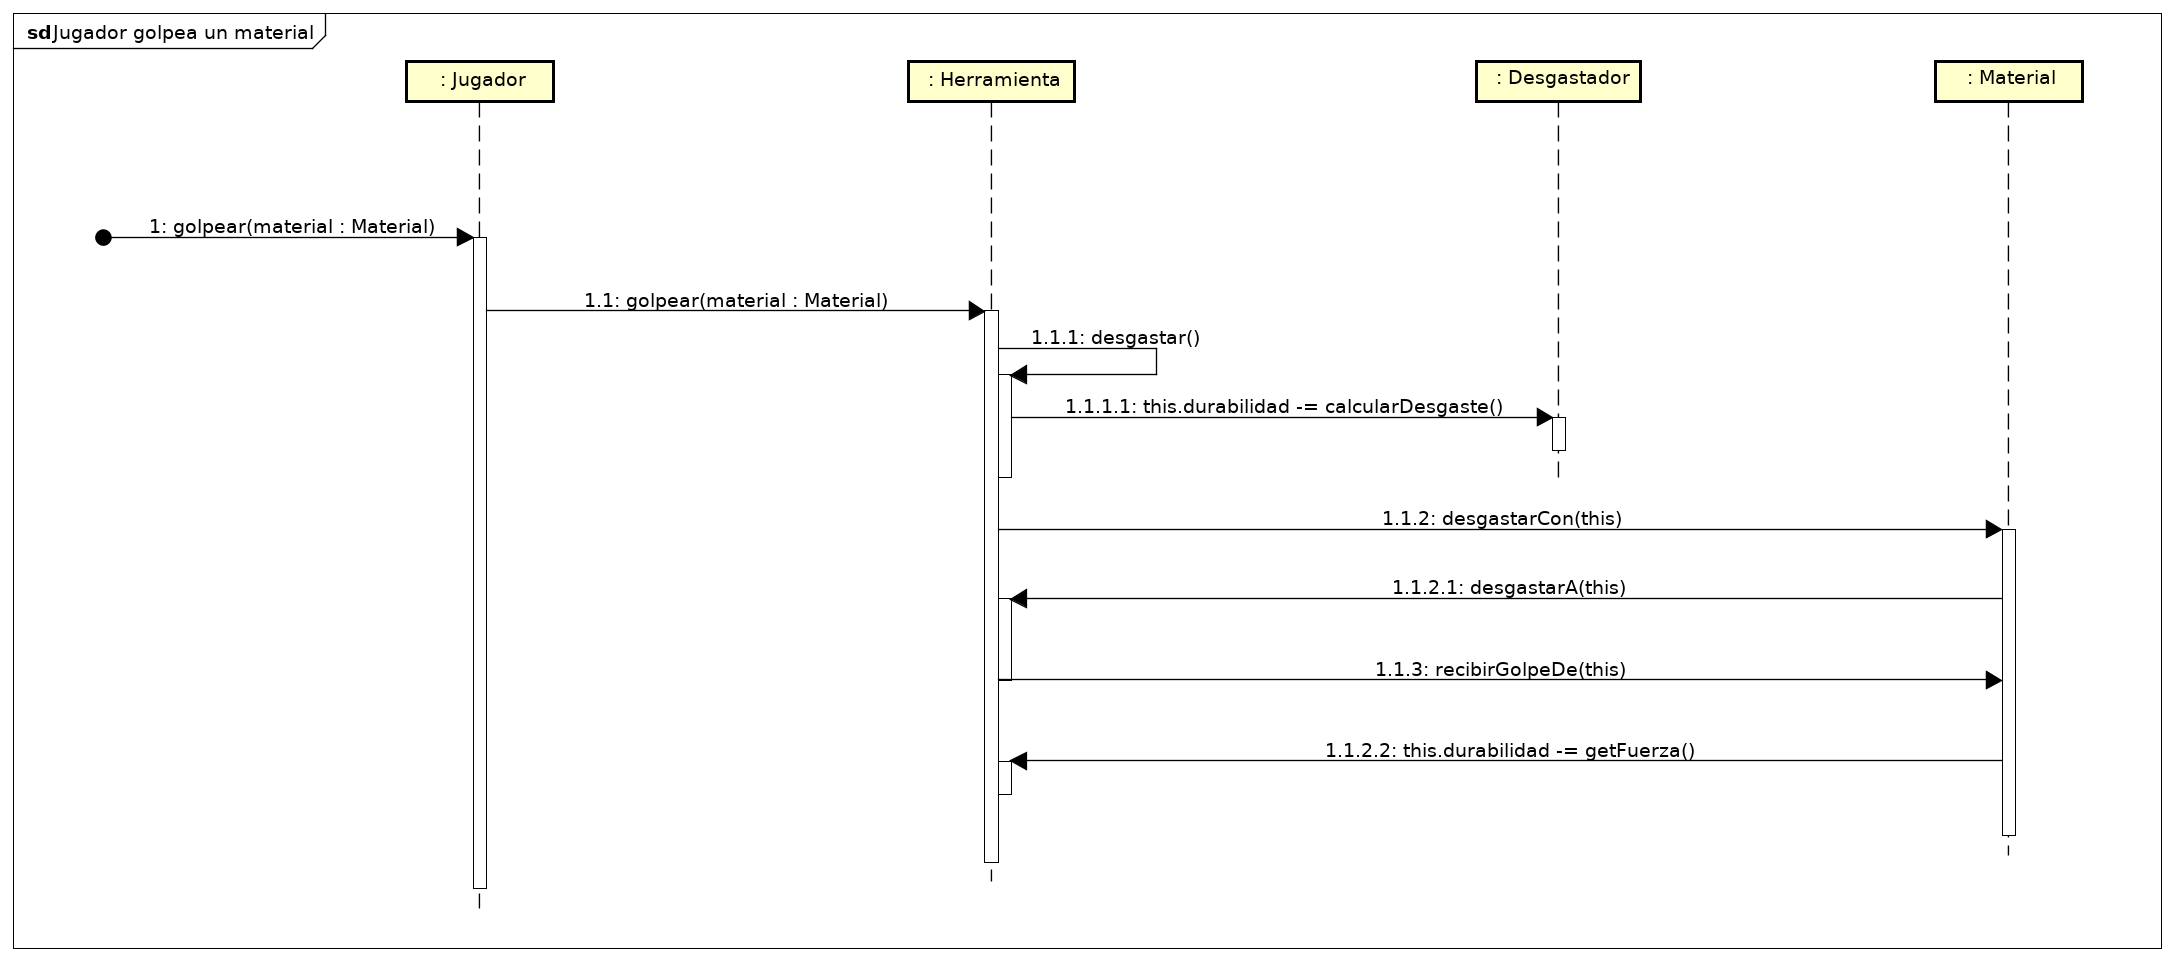
\includegraphics[width=\textwidth]{Diagramas/JugadorGolpeaMaterial.png}
\caption{\label{fig:jugadorGolpeaMaterial}Jugador golpea un material.}
\end{figure}

\begin{figure}[H]
	\centering
	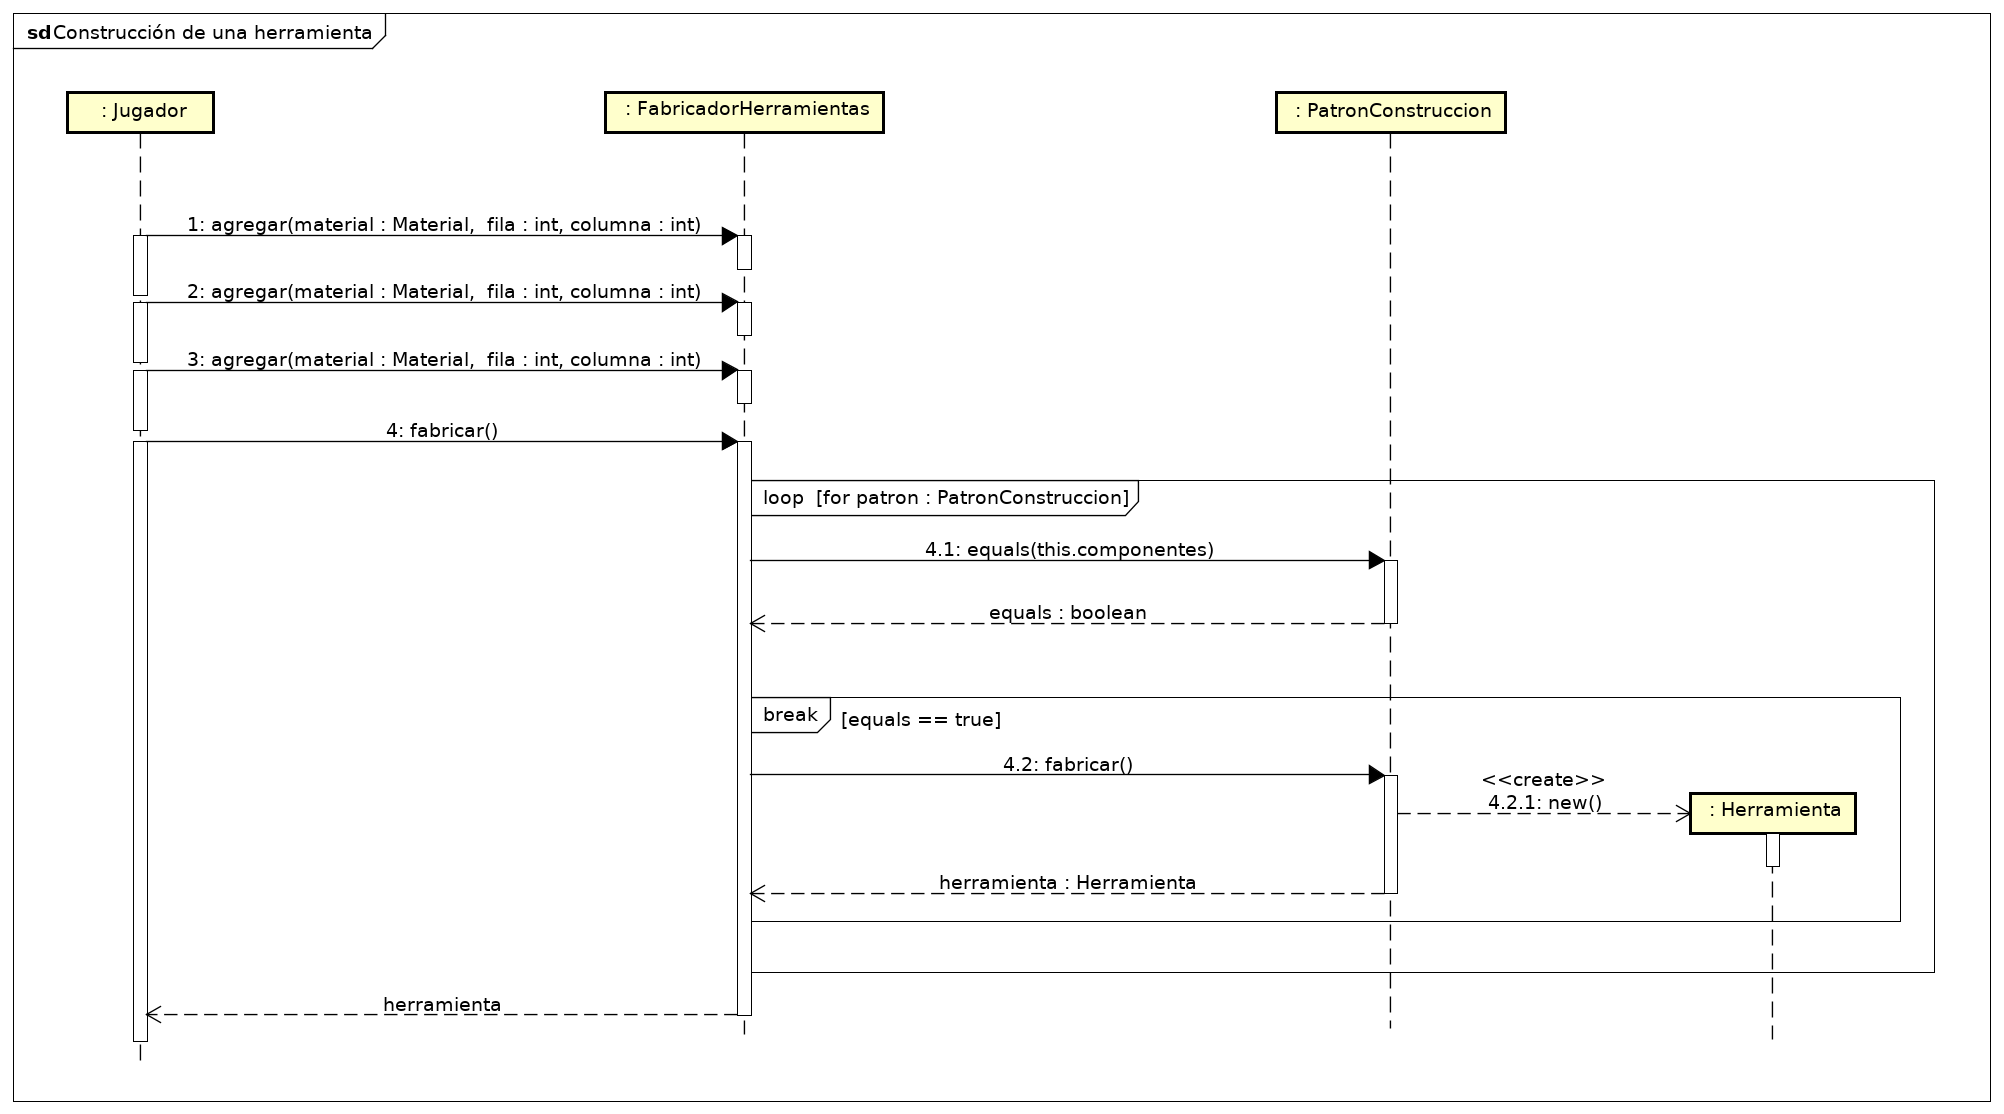
\includegraphics[width=\textwidth]{Diagramas/ConstruccionHerramienta.png}
	\caption{\label{fig:fabricacion}Construcción de una herramienta.}
\end{figure}


\section{Diagrama de estados}\label{sec:diagramadeestados}
\begin{figure}[H]
	\centering
	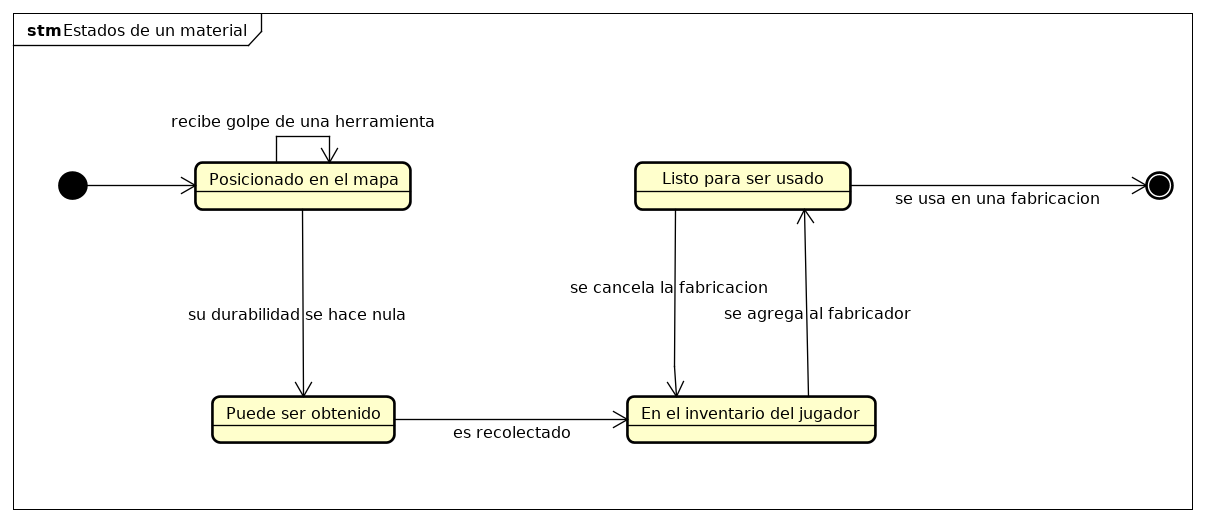
\includegraphics[width=\textwidth]{Diagramas/EstadosMaterial.png}
	\caption{\label{fig:estadosmaterial}Diagrama de estados de un material.}
\end{figure}

\begin{figure}[H]
	\centering
	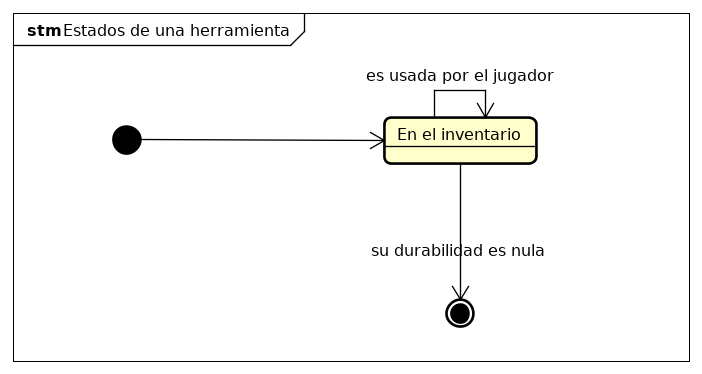
\includegraphics[width=0.7\textwidth]{Diagramas/EstadosHerramienta.png}
	\caption{\label{fig:estadosherramienta}Diagrama de estados de una herramienta.}
\end{figure}

\begin{figure}[H]
	\centering
	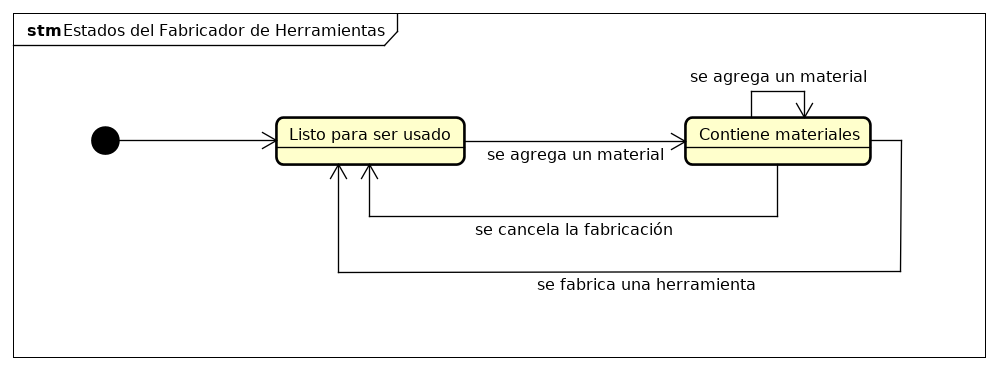
\includegraphics[width=\textwidth]{Diagramas/EstadosFabricador.png}
	\caption{\label{fig:estadosfabricador}Diagrama de estados del fabricador.}
\end{figure}

\section{Diagrama de paquetes}\label{sec:diagramadepaquetes}
\begin{figure}[H]
	\centering
	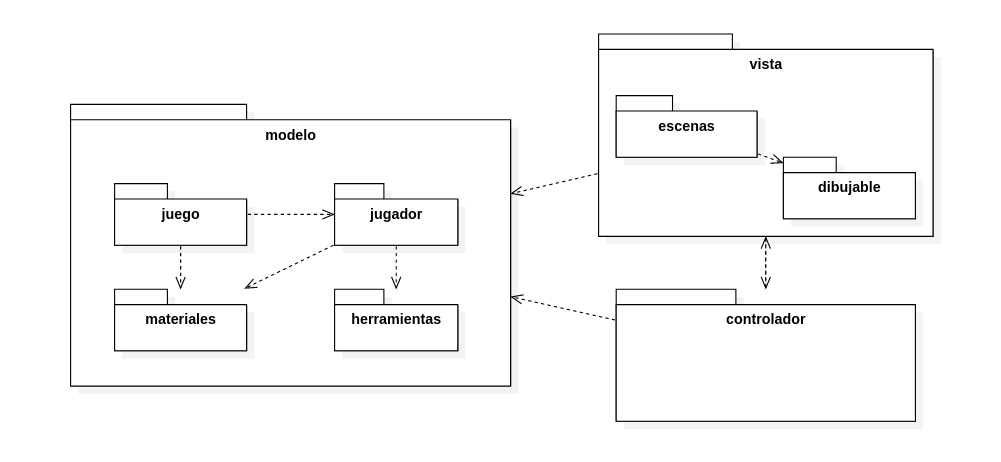
\includegraphics[width=\textwidth]{Diagramas/Paquetes.png}
	\caption{\label{fig:paquetes}Diagrama de paquetes del trabajo práctico.}
\end{figure}

\end{document}